\chapter{Implementation and evaluation}
\label{cha:results}
This chapter will present how the system was developed, giving a panoramic view of the interaction between components and a detailed focus on the solution chosen to deal with external services with a limited number of requests in a certain time range. After that, the development techniques for the classifier will be presented, along with the performance evaluation of the latter one, and finally an evaluation about the detection process will be provided.

\section{Component interactions and communications}
\label{sec:view}
\begin{figure}
\centering
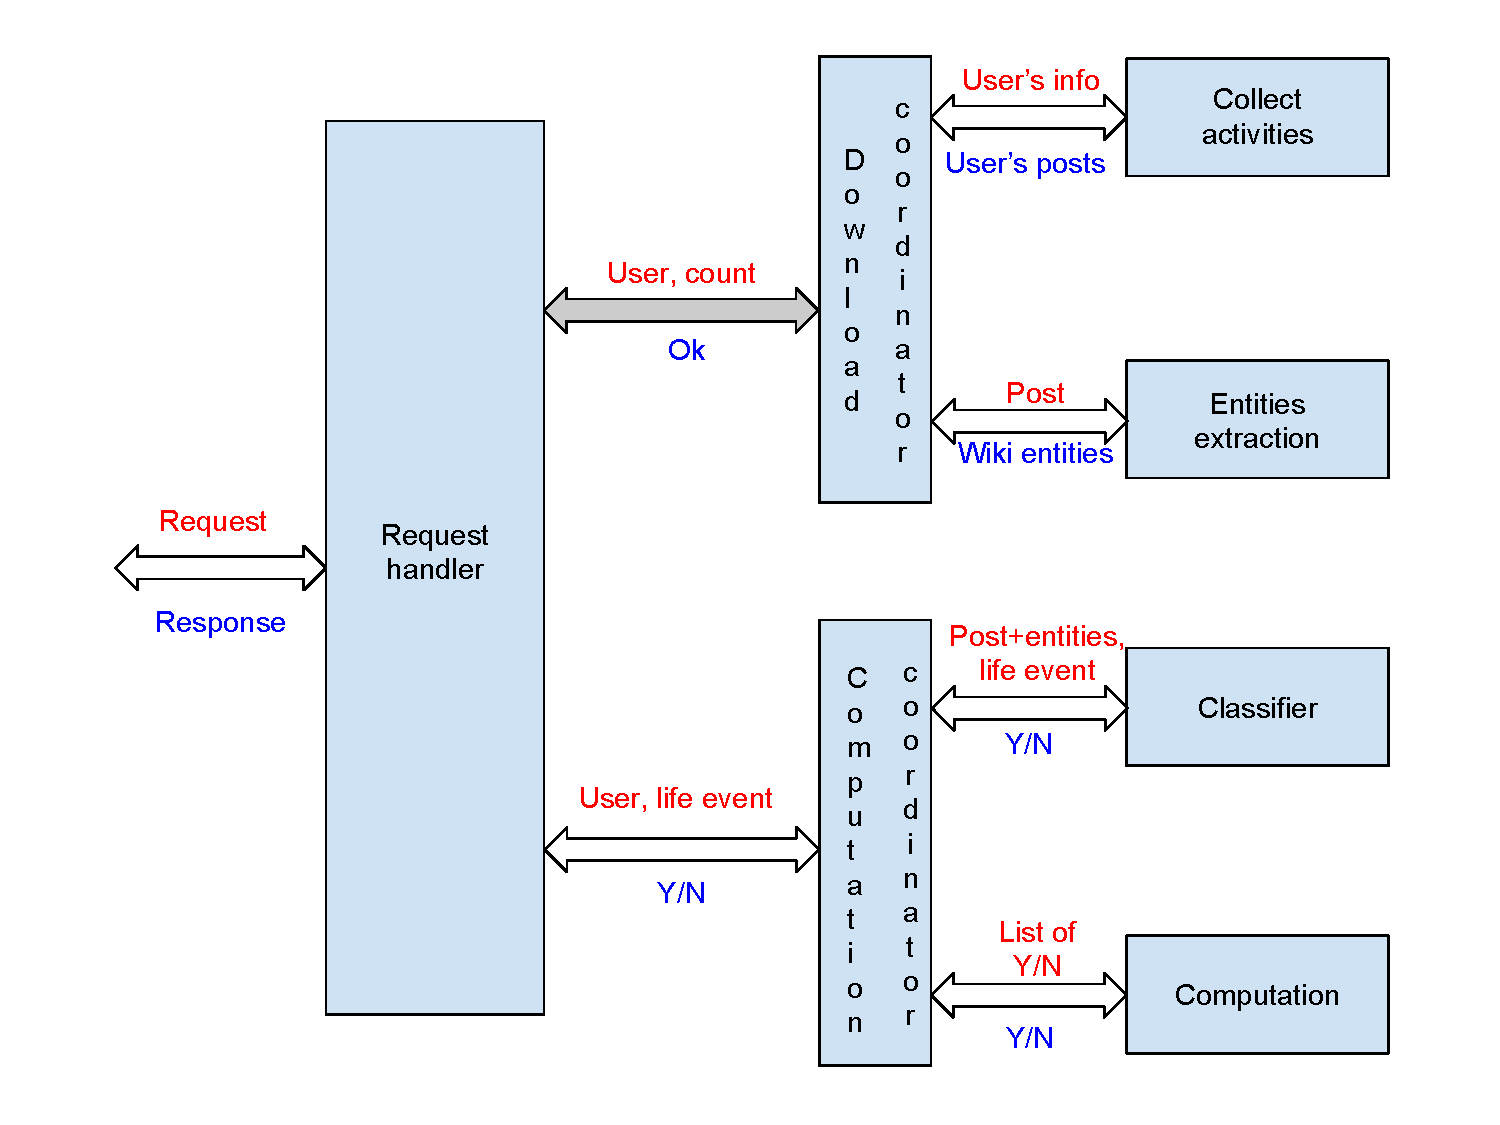
\includegraphics[width=%
1.0\textwidth]{img/Globalview}
\caption{A global view of the system with the data exchanged between the components. Grey arrows are queues of inputs, while white arrows are messages of a class method call.}
\label{fig:globalview}
\end{figure}

Overall, the whole system can be divided in two big parts: the one to get the data, the other to analyze them. The four logical steps previously explained in section~\ref{sec:logicdescr} are translated into four components placed in the deepest point of each request, as shown in figures~\ref{fig:globalview} and \ref{fig:interaction}. These four parts have different roles and behaviours: some of them are autonomous, while some others depend one from the other. Each one provides its own API, as shown in section~\ref{sec:apis}, to allow the system to be scalable.

\begin{figure}
\centering
\includegraphics[width=%
1\textwidth]{img/Interaction}
\caption{The interaction among components over time.}
\label{fig:interaction}
\end{figure}

The request handler is the user's endpoint of the system, the only access point from the outside. This component allows managing the addition and modification of the users to be analyzed, and starts a content download or a computation of the timeline.

The download request will be described in detail in section~\ref{sec:downloadqueues}.

The computation request is much easier, because it only works with data within the system, without any external service. Each request is fulfilled with the personal data of the user in analysis present at the moment of the request. This process can be seen in the lower part of picture~\ref{fig:globalview}. User's posts are firstly classified as related or not to the life event taken into analysis, and then data is given to the computator part to detect the life events into user's timeline, as explained in section~\ref{sec:computation}. 

\subsection{A queue system to download user's contents}
\label{sec:downloadqueues}

\begin{figure}
\centering
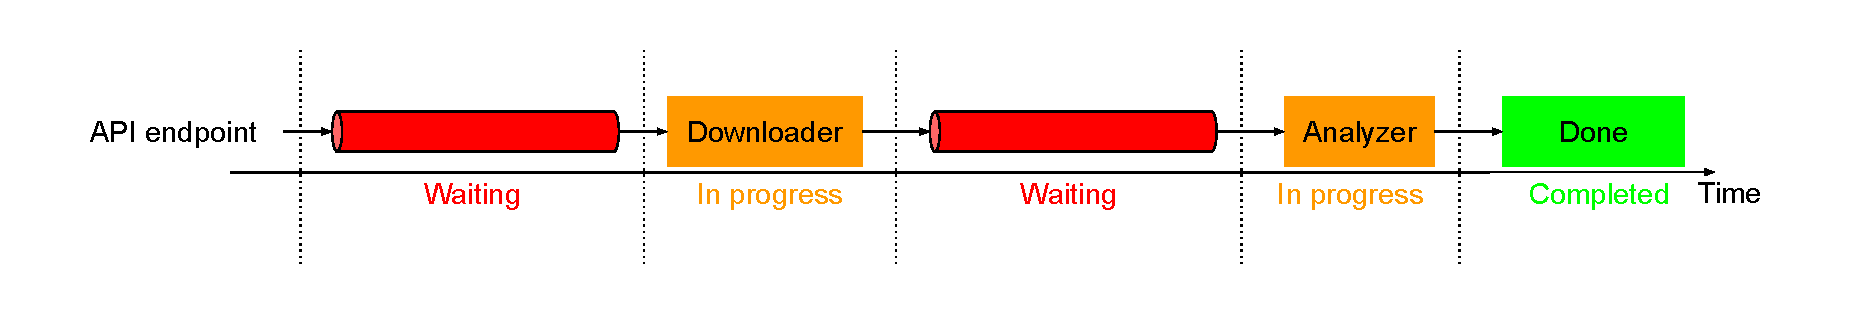
\includegraphics[width=%
1\textwidth]{img/DownloadStatuses}
\caption{The changing of status over time of a download request.}
\label{fig:statuses}
\end{figure}

\begin{figure}
\centering
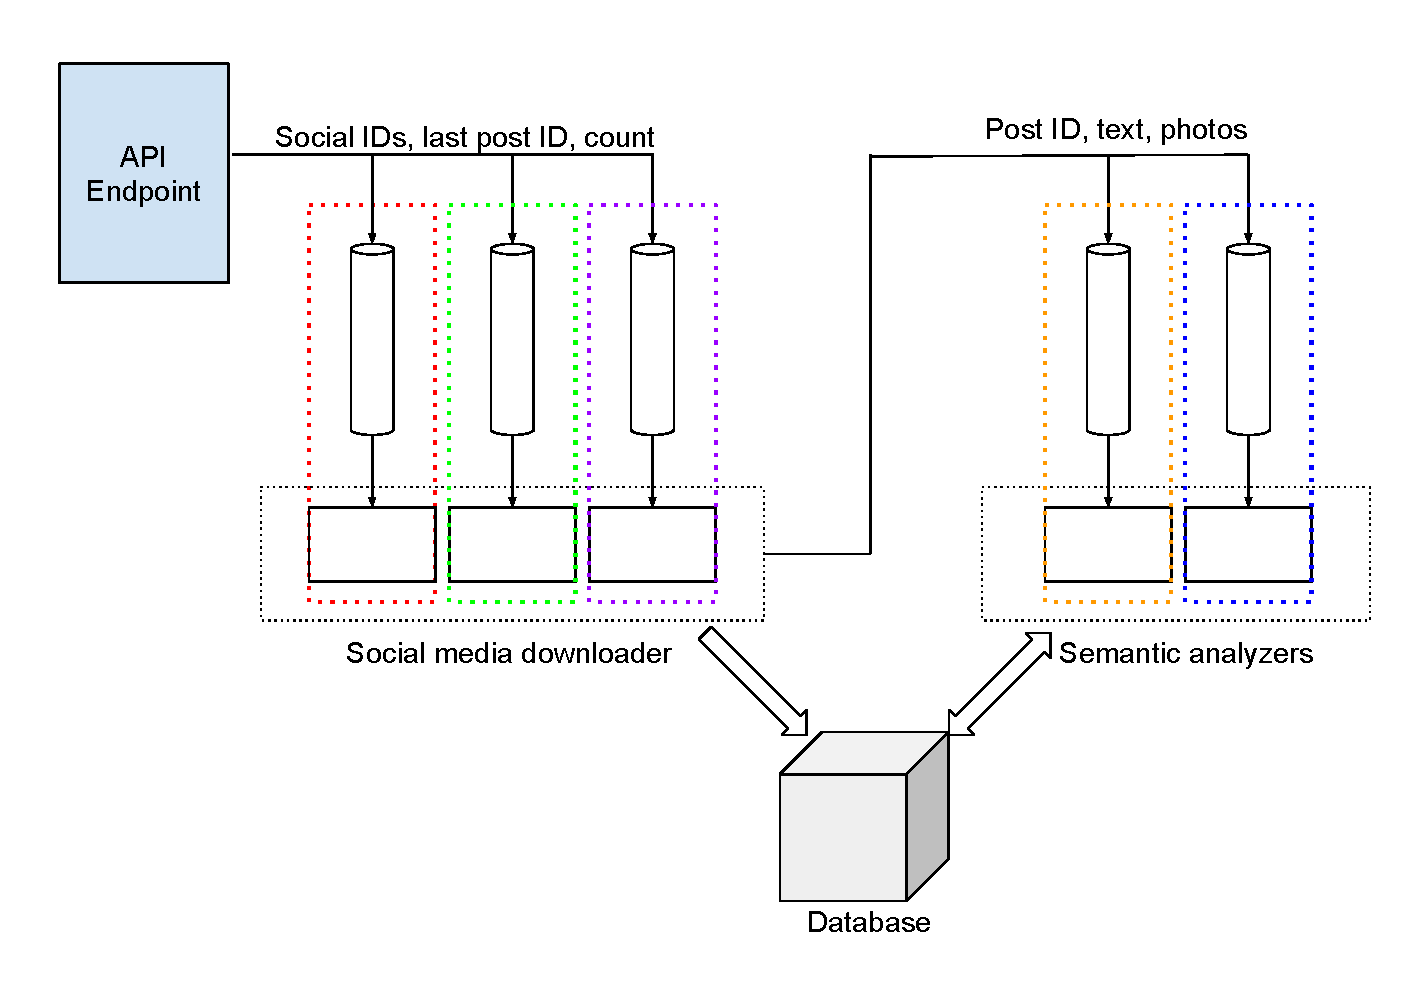
\includegraphics[width=%
0.85\textwidth]{img/Queues}
\caption{The route of a download request. From the endpoint, data is divided in independent streams, one for each social media, and each stream is enqueued in the corresponding queue. The red, green and purple frames represents three different social network download system -- for example the red one for Facebook, the green one for Twitter and the purple one for Instagram. Once data is downloaded, it is saved into the database, and posts are given to the semantic analyzers, represented by the orange and blue frames: one for texts and one for images.}
\label{fig:queues}
\end{figure}

The most complex request is a \texttt{/downloadrequest}, because it has to face itself with external APIs over HTTPS, which have free plans with some request limits over a time range. Due to this issue, each part needed to fulfill this kind of requests has to be able to suspend itself without interrupt the whole system in case request number runs out. In other words, when the function for downloading contents on a social network, or the one that deals with the external semantic analyzer reaches the limit of requests, it has to wait for another time slot stopping only itself and nothing else. For this reason data is not passed with a standard class method call, but it's inserted into a queue. There will be a queue for each module that has to interface itself with an external service, so one for each social media and one for every semantic analyzer (one for texts and one for pictures). This decision is necessary to avoid bottlenecks as much as possible: in case a social network API reaches the limit, the downloads in the other social networks can be carried on, and so also the following requests can start. The only thing that is necessary is to track when each part of the Download Request finishes, in order to have always a current status for every request of download: when at least a data stream of a request is taken over by some downloader or analyzer, the status is \emph{in progress}, while if all data streams of a requests are waiting into a queue, the status is \emph{waiting}. By the time each stream passed into its specific downloader and analyzer successfully, the status will be \emph{completed}. The status timeline can be seen in picture~\ref{fig:statuses}.

For example, let's suppose to download contents made by a user who is signed up to Twitter, Facebook and Instagram. The request will be collected by the API endpoint, which will verify if the user exists into the database of the system, and in case it exists the endpoint will get from the same database, for each of the three social media, the user ID on that social network and the last post downloaded in a previous request, if there is one. After that, the tuple (user ID, starting point, number of post to download) is queued in the respective social media queue, and an immediate response is given to the API request, to let the user know that her request has taken into consideration. At this point, three stream of data (one for each social media) are created, and they will go on independently: each of them will wait its turn into the downloader queue, then data will be downloaded and saved into the database. At this point other two streams for each downloaded post are created, one for images and one for texts: the tuples (post ID, text) and (post ID, photos) will be enqueued in the text semantic analyzer and in the image semantic analyzer respectively. When all these streams will have passed both downloader and analyzers, the request will be completed. This schema can be seen in picture~\ref{fig:queues}.

Even though this architecture avoids as much as possible bottlenecks, a download request can take a very long time to be completed (even days), because each post from any social media has to pass through the semantic analyzers, which have a very restricted number of requests a day.

\section{Implementation choices}
\label{sec:choices}
Due to the recent Cambridge Analytica scandal that involved Facebook, and with the consequent policy updates made by the social network, develop an application that works with Facebook products (Facebook itself and Instagram, for instance) that uses user's contents has become difficult. To do that, Facebook has to release a manual authorization after a demo video has been created to show what the application does. Even if a beta development had been used, it would have been hard to find enough users available to share their data for the development of this system. For these reasons it was decided to base the application on Twitter.

Another issue is related with the external semantic analyzers: only free account has been used, which implies a very strict number of requests per day (1000). This means that currently a computation can take a very long time to be executed, even days, because each post has to be analyzed by this external services. Furthermore, image analyzers have free plan with only 1000 request a month, so it was decided to use only texts of posts, and to ignore images. All the obtained result, therefore, are only related with texts of tweets. On the other hand, some tests with images were executed, showing that the use of images would give better results: in fact, several posts of life events are composed only by images, so at the current situation they can't be classified correctly.

About implementation, the system is developed in Python, using some standard libraries for machine learning and mathematical purposes: the classifiers  
are those available in the \texttt{scikit-learn}\footnote{\url{scikit-learn.org}} library \cite{scikit-learn}, while for numerical arrays, matrices and other mathematical functions the \texttt{NumPy}\footnote{\url{www.numpy.org}} library \cite{oliphant2006guide} is chosen. Data is stored and organized using a \texttt{MongoDB} database\footnote{\url{www.mongodb.com}}. Last but not least, the external semantic analyzer for texts is called \texttt{Dandelion}\footnote{\url{dandelion.eu}} made by SpazioDati S.r.l.\footnote{\url{spaziodati.eu}}. Some test with images were also performed, using the \texttt{Cloud Vision API} of Google Cloud\footnote{\url{cloud.google.com/vision}}.

\section{Feature extraction}
\label{sec:featurextraction}
In this section the feature extraction technique will be presented. It is thought to work with posts from various social networks, whose structure can be seen in section~\ref{sec:apis}. In general, each post has a text and a series of images that are used for the classification. According to section~\ref{sec:dataset}, Wikipedia entities are used as features, for two reasons:
\begin{enumerate}
\item In this way it's possible to work with as many languages as is wanted, using only one for training. In fact, letting $ L $ be the language of the samples in the training set, it's enough to map all the entities found in posts written in a language $ L^{'} \ne L $ to the corresponding entity in the $ L $ version of Wikipedia. All the most common entities for life events exist in many version of the online encyclopedia.
\item With this method is possible to consider texts and images in the same way, seeing them as \emph{entity containers} without differentiating them.
\end{enumerate}

The feature extraction is done in this way: each entity of the samples of the training set is kept as feature, and a matrix $X$ is created, with $n$ rows, one for each sample to classify, and $m$ columns, one for each feature. Each element [$i,j$] of $X$ is the counter of how many times the entity $j$ is found in the post $i$. The number $m$ of columns is in the order of thousands.

Of course, the features used for weddings is different than the one for births, and consequently two different machine learning classifiers are needed, each one trained for its specific life event. To do that, the dataset taken from \cite{dickinson2015identifying} was filtered, keeping only tweets about a wedding or a birth of a child. Then it was splitted in two files, one for each life event, and every tweet was enriched with Wikipedia entities and topics using the external semantic analyzer. In the end, the wedding dataset counted $2538$ samples, the births one $2233$. Each of these sets were very balance, with half of the sample related to the life event and the other half not. Both datasets were then used to train each classifier.

\section{Construction and performance evaluation of the classifier}
In this section all the techniques used to create a classifier as good as possible will be explained.

 According to the literature, a naive bayes classifier and a decision tree were chosen as classifiers, but due to the better performance of the first one, the second one was initially discarded. In particular, the classifier was a Multinomial Naive Bayes\footnote{\url{scikit-learn.org/stable/modules/naive_bayes.html#multinomial-naive-bayes}}.

The very first feature extraction technique was inspired by the \texttt{tf-idf} weight function\footnote{\url{en.wikipedia.org/wiki/Tf–idf}}, which is used to understand the importance of a word into a series of documents. The idea was to select a small sample of key entities analyzing some web pages focused on the life event taken into consideration, such as a wedding planner homepage or a pregnancy blog. These $k$ top entities were used as features of tweets, and a matrix $X$ was created in the same way explained in section~\ref{sec:featurextraction}, but with $m = k$. However, this methodology performed worse than a random classifier, with both precision and recall scores lower than $0.5$, with $k = 3, 4, 5, 10, 100$.

\begin{table}[htbp]
\centering
\subtable[Results on a single dataset split\label{tab:singlesplit}]{%
\begin{tabular}{cccc}
\hline
Life event & Precision & Recall & F1 Score \\
\hline
\textbf{Getting married} & $0.82$ & $0.81$ & $0.81$ \\
\textbf{Having children} & $0.77$ & $0.78$ & $0.77$ \\
\hline
\end{tabular}
}\qquad\qquad
\subtable[Results on a 10 fold cross validation\label{tab:kfold}]{%
\begin{tabular}{cccc}
\hline
Life event & Precision & Recall & F1 Score \\
\hline
\textbf{Getting married} & $0.73$ & $0.82$ & $0.77$ \\
\textbf{Having children} & $0.62$ & $0.57$ & $0.59$ \\
\hline
\end{tabular}
}
\caption{The performance of the naive bayes were satisfactory on a very balanced dataset. Unfortunatly, users' timelines are very unbalanced, and this classifier turned out to be inappropriate.}
\end{table}

A much better performance with the dataset, but unfortunately not with the reality, was given by using all the Wikipedia entities of the training set as features, exactly as explained in section~\ref{sec:featurextraction}. Firstly, the dataset was splitted into a training and a test set, the first one with the 70\% of the samples and the second with the remaining 30\%; secondly, the matrix $X$ was created. On the test set this solution had good results, as shown in tables~\ref{tab:singlesplit} and \ref{tab:kfold}, but in the reality, trying to predict if tweets from a user timeline were about or not a life event, this solution turned out to be impractical: the discrimination was too loose, and many tweets that wasn't related with the life event at all were considered "positives", with the precision measure that fell dramatically under $0.1$. The overfitting reason was excluded, because the training set was kept aside from everything else. In addition, each sample in the dataset was written by a unique user. The most probable reason is that the dataset used for the training was too balanced compared to the real situation in social networks: in fact, while the dataset contained about 50\% of tweets about a life event and 50\% not, a timeline had a very small percentage of contents about a life event. For example, analyzing a portion of Gareth Bale's Twitter profile\footnote{\url{twitter.com/GarethBale11}}, it turned out that on 224 tweets only 2 were about the birth of a child and only one about marriage. Many other profiles considered had similar proportions.

A third approach was tried, with the purpose of improve the previous situation: train the classifier with a very unbalanced dataset, discarding randomly many of the positive samples to create a 90\% negatives and 10\% positives situation. In each test the positive subset were different, because of randomness, but as before the results were good only with the test set: with a real profile the discrimination was too strong this time, not finding any tweet at all, maybe just because of this disproportion, where too few related samples were given and so the classifier didn't see enough entities among those of positive samples.

Another very big issue was caused by the external semantic analyzer - Dandelion - used to discover Wikipedia entities inside texts. Its results turned out to be very inaccurate for such short texts written in Twitter: for example, a tweet published by a famous sports man about his wedding, with the text "\textit{This is her, my wife}"\footnote{\url{twitter.com/petosagan/status/667069250268479488}} was mapped by the analyzer to a song by the British rock band \emph{the Who} called \emph{My Wife}, not understanding the context at all. Some other cases of misunderstanding between the text and its true meaning were found, for example the word \emph{congratulations} was mapped into the entity "\texttt{Congratulations: 50 Years of the Eurovision Song Contest}", but this was not a big issue because this combination was always respected every time that word was found. Just to be sure that some words were recognized correctly, 4 keywords for each event were manually mapped into their correct entities, such as \emph{baby} on the entity \texttt{Infant}.

\begin{sidewaysfigure}
\centering
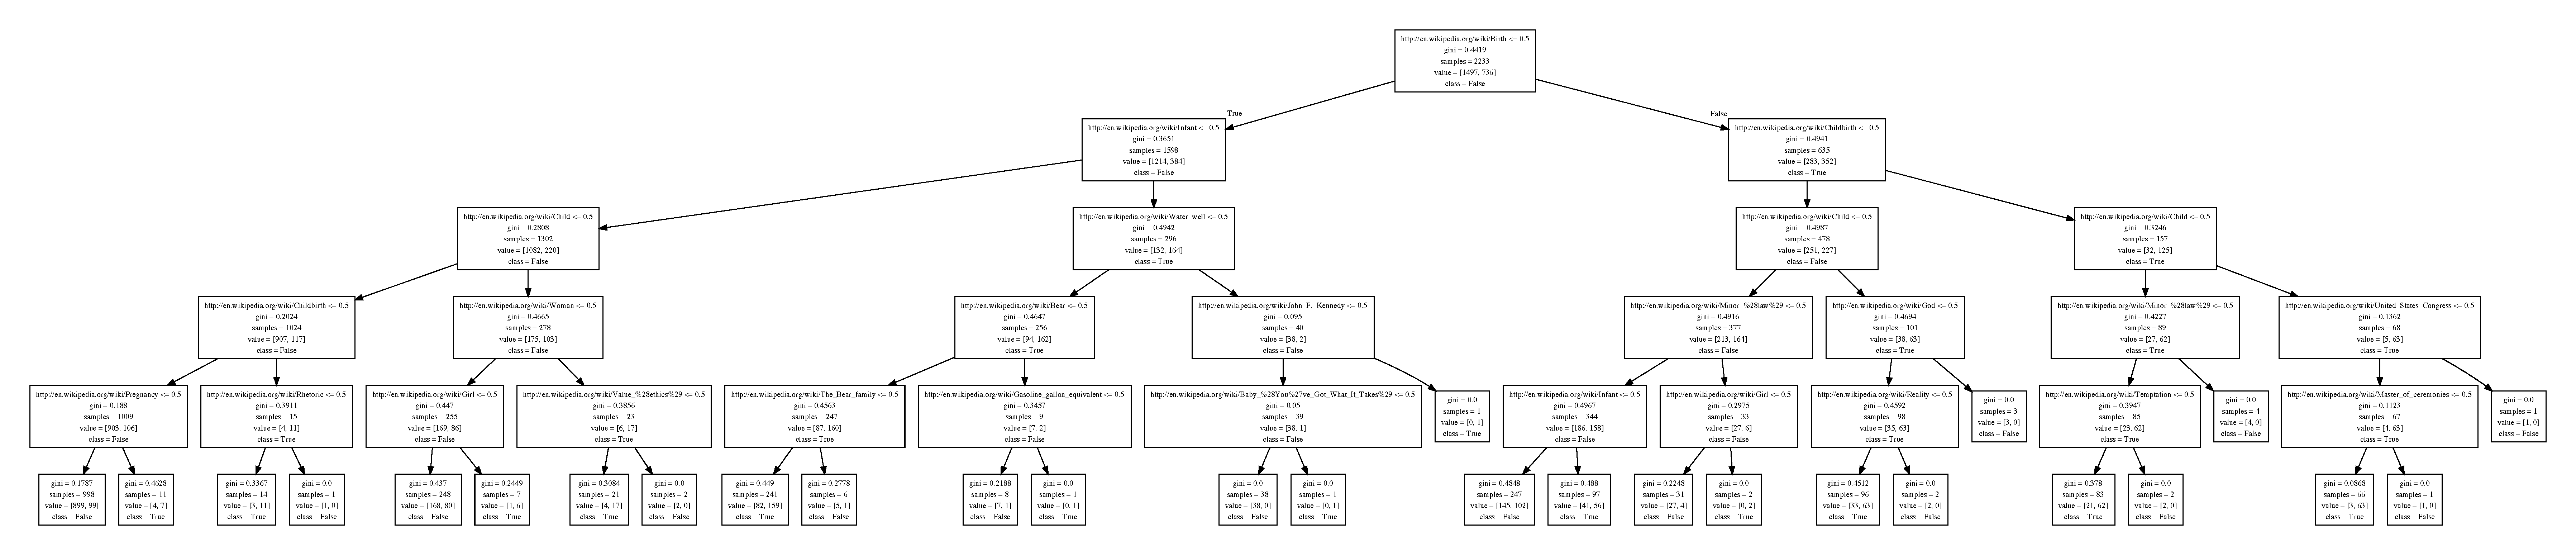
\includegraphics[width=%
1\textwidth]{img/decisiontree}
\caption{The decision tree for the birth of a child event. As can be seen, the nearest nodes to the root are decisions about entities that are strictly connected with the life event itself, and each of them makes a significant split in terms of the size of the resulting subsets, while the deepest nodes are strongly connected with the training set. For this reason the maximum depth was forced to be low.}
\label{fig:decisiontree}
\end{sidewaysfigure}

To avoid issues with the semantic analyzer as much as possible, as few as possible entities were used to classify a tweet: a very first approach consisted in a manual selection of features, for example the entity \texttt{Wife} for wedding, but the results were not satisfactory. The definitive approach was to let the data decide which entities to use, relying on the dataset taken from \cite{dickinson2015identifying}. The classifier was changed, opting for a decision tree, because the previous naive bayes was too loose during the classification. A decision tree is a machine learning model used for regression and classification based on a binary tree data structure. Each node of the tree is a question relative to a feature of the objects to classify, and each leaf represent a decision, an estimation of the value of the input object. During the training, the tree is build starting from the root: at each step of the construction, the goal is to split the dataset into two, making a question on a feature of the objects, to reduce the unpredictability of the two new subsets as much as possible. Every object in input will have its path from the root to a single leaf, which will represent the decision. Precisely, the classifier was the decision tree offered by the \texttt{scikit-learn} library\footnote{\url{scikit-learn.org/stable/modules/generated/sklearn.tree.DecisionTreeClassifier.html}}. To reduce the overfitting on the training data, the maximum depth of the tree was limited to 5, so for each root-leaf path, at most 4 intermediate nodes could be found. The decision tree for the life event \texttt{Having Children} can be seen in figure~\ref{fig:decisiontree}.

To further improve the results and to make sure that some key entities are identified, an automatic check on the texts of the posts is done. In particular, for each life event $LE$ and for each language $L$, a set of keyword translation $T(LE, L)$ is defined. For example, for the life event \texttt{Having children} and for the english language, $T$ is so defined:
\begin{equation*}
\begin{split}
T(\text{\texttt{Having children}}, \text{english}) = \{&(\text{"birth"}, \text{ \texttt{\url{http://en.wikipedia.org/wiki/Birth}}}),\\&(\text{"born"}, \text{ \texttt{\url{http://en.wikipedia.org/wiki/Birth}}}),\\&(\text{"baby"}, \text{ \texttt{\url{http://en.wikipedia.org/wiki/Infant}}}),\\&(\text{"child"}, \text{ \texttt{\url{http://en.wikipedia.org/wiki/Child}}})\}
\end{split}
\end{equation*}

The results with the dataset of \cite{dickinson2015identifying} were a little worse than those of the bayesian classifier shown in tables~\ref{tab:singlesplit} and \ref{tab:kfold}, but in the reality, with a test conducted on 5836 tweets taken by 43 different timelines the results were much better than the previous one, as explained in tables~\ref{tab:treewedding} and \ref{tab:treechild}.

\begin{table}[htbp]
\centering
\subtable[Results about wedding tweets\label{tab:treewedding}]{%
\begin{tabular}{ccccc}
\hline
Sample & Precision & Recall & F1 Score & Support \\
\hline
\textbf{True} & $0.87$ & $0.70$ & $0.77$ & $134$ \\
\textbf{False} & $0.91$ & $0.97$ & $0.94$ & $5702$ \\
\textbf{Avg / Total} & $0.90$ & $0.90$ & $0.90$ & $5836$ \\
\hline
\end{tabular}
}\qquad\qquad
\subtable[Results about birth of a child tweets\label{tab:treechild}]{%
\begin{tabular}{ccccc}
\hline
Sample & Precision & Recall & F1 Score & Support \\
\hline
\textbf{True} & $0.65$ & $0.62$ & $0.63$ & $161$ \\
\textbf{False} & $0.93$ & $0.94$ & $0.94$ & $5675$ \\
\textbf{Avg / Total} & $0.89$ & $0.89$ & $0.89$ & $5836$ \\
\hline
\end{tabular}
}
\caption{The performance of the decision tree with a very unbalanced dataset. On this same test set the previous classifier, the naive bayes, showed both precision and recall scores under 0.1.}
\end{table}

\section{Detection evaluation}
\label{sec:detectioneva}
\noindent
\renewcommand\arraystretch{1.5}
\setlength\tabcolsep{0pt}
\begin{table}
\centering
\subtable[Getting married\label{tab:weddingconf}]{
\begin{tabular}{c >{\bfseries}r @{\hspace{0.7em}}c @{\hspace{0.4em}}c @{\hspace{0.7em}}l}
  \multirow{10}{*}{\parbox{1.1cm}{\bfseries\raggedleft Actual\\ value}} & 
    & \multicolumn{2}{c}{\bfseries Prediction outcome} & \\
  & & \bfseries True & \bfseries False & \bfseries Total \\
  & True & \MyBox{4}{} & \MyBox{0}{} & 4 \\[2.4em]
  & False & \MyBox{4}{} & \MyBox{15}{} & 19 \\
  & Total & 8 & 15 &
\end{tabular}
}
\quad
\subtable[Having children\label{tab:childrenconf}]{
\begin{tabular}{c >{\bfseries}r @{\hspace{0.7em}}c @{\hspace{0.4em}}c @{\hspace{0.7em}}l}
  \multirow{10}{*}{\parbox{1.1cm}{\bfseries\raggedleft Actual\\ value}} & 
    & \multicolumn{2}{c}{\bfseries Prediction outcome} & \\
  & & \bfseries True & \bfseries False & \bfseries Total \\
  & True & \MyBox{10}{} & \MyBox{0}{} & 10 \\[2.4em]
  & False & \MyBox{9}{} & \MyBox{3}{} & 12 \\
  & Total & 19 & 3 &
\end{tabular}
}
\caption{Confusion matrices of boolean tests}
\end{table}
Before presenting the results about the detection method it's right to make a premise. The results that will be showed now are obtained using data that are composed only by texts coming from Twitter. For this reason they are not excellent but they have an ample room for improvement.

First of all, the tests were executed with 30 different Twitter accounts, some of them completely downloaded, some other only partially. Totally, 19 of them had children in their real life and shared something about it, 8 got married and shared something too, some of these lived both a marriage and a birth of a child, and one of them had two children. In addition to that, some other account that was not concerned with these two life event were added to the samples. Not all the 30 accounts were tested on both life events.

Secondly, two types of tests were made:
\begin{itemize}
\item A boolean valuation without consider the temporal factor, that indicates whether the detection reflects the fact that the subject of the analysis really experienced that event in his life.
\item An evaluation on the quality of the time ranges returned.
\end{itemize}
For the first test, which is the classic test usually done with a classification problem, the results can be seen in the two confusion matrices, \ref{tab:weddingconf}~for weddings and \ref{tab:childrenconf}~for births respectively.

For further details, the following are the results for wedding cases,
\begin{gather}
Accuracy = 0.83 \quad Precision = 1.0 \quad Recall = 0.5 \quad F_1\text{-}Score = 0.67
\label{weddingconfdata}
\end{gather}
and for births of child
\begin{gather}
Accuracy = 0.59 \quad Precision = 1.0 \quad Recall = 0.53 \quad F_1\text{-}Score = 0.69
\label{childrenconfdata}
\end{gather}
respectively.

